\section{Practical Security} \label{sec:practical-security}

% 🥚 EASTER EGG: This is where theory meets reality, and reality is messy
% Theory: "Assume a spherical cow in a vacuum"
% Practice: "The cow is actually a malicious adversary in disguise"

Our theoretical guarantees assume that the local computer is completely trusted. Nothing can defend against a preinstalled backdoor, so we can never eliminate client-side risk, but we \textit{can} reduce it. This section outlines the mitigations we undertake: reducing the attack surface through modularization and supply chain protection, open-sourcing our client, securing code distribution and updates, and protecting against non-privileged local malware.

We emphasize that we can never eliminate client-side risk. \textbf{PLEASE DO NOT USE ANYSPHERE FOR SECURITY-CRITICAL USE CASES ON A COMPUTER YOU DO NOT TRUST}. This is especially true while we are in beta, and may have bugs.

% 🥚 EASTER EGG: Translation: Don't use this for planning your surprise birthday parties on your work laptop
% 🥚 EASTER EGG: "may have bugs" = definitely has bugs, we just haven't found them all yet

% The Anysphere client is only as strong and secure as the most vulnerable part of our software supply chain. Software supply chains are an increasingly complex (and brittle) part of the software ecosystem because of a large and growing number of direct and transitive dependencies written across the world. 
% The Anysphere client is designed to handle extreme private and critical communication securely, so our team has enforced a high bar of security for the core of our system. We focused on providing practical protection by significantly reducing the attack surface of our client, ensuring safe updates, and protecting against non-privileged software. 

% A note on the client's security, in the context of our threat model: Anysphere trusts its client's devices. 
% In particular, we trust that the local device is running a correct implementation of our protocol, and the computer comes without pre-installed backdoors. 
% Our model is the bare minimum of trust we must assume, and we think this is reasonable given the intense focus of Apple and many other companies on device security. 
% (Put another way, no encryption schemes we can come up with can secure our client inside a compromised computer.)
% And with this context, we will present our measures to reduce the risk of a compromised Anysphere client.


\subsection{Reducing the attack surface}

As illustrated in \cref{fig:systemdiagram}, our client consists of two parts: a UI frontend and a daemon backend. We sandbox the UI so that it is not allowed to talk to the internet. Instead, all communication goes through the daemon, which contains all security-critical code. Thus, bugs and malicious code on the frontend have a harder time compromising security.
\begin{figure}[t!]
    \centering
    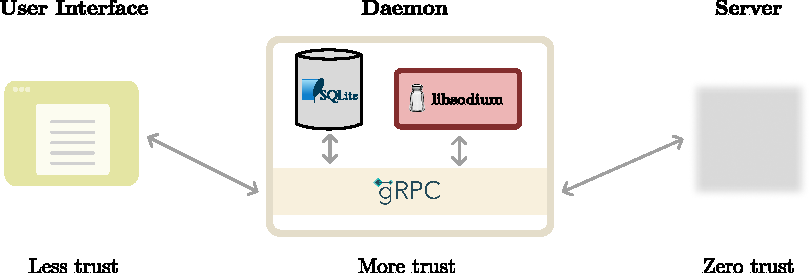
\includegraphics[width=\textwidth]{sysdiagramalt.pdf}
\caption{System architecture. The UI and the daemon run on your local computer and require some trust assumptions. The UI is cut off from the internet, and can only communicate via the daemon, meaning that it needs lower trust assumptions. The crypto module in the daemon requires the highest level of trust.}
\label{fig:systemdiagram}
\end{figure}

We also reduce the attack surface of the daemon. In particular, we ensure a small dependency chain to prevent supply chain attacks. We chose to use \Cpp for all essential daemon code, depending only on a few well-known packages with long-term support and good security practices (Abseil, gRPC, SQLite, Libsodium). We wrote a Rust API for database interactions, being extremely careful with our dependency chain. 

% Many popular languages, including Rust, Go and Python, have great package managers, which led to an ecosystem where packages generally have hundred of transitively dependencies. <- no need to emphasize this?

\subsection{Open source}

All code that is required for security is open source. The repositories \\ {\tt \href{https://github.com/anysphere/client}{github.com/anysphere/client}} and  {\tt \href{https://github.com/anysphere/asphr}{github.com/anysphere/asphr}} contain all code for our daemon and UI. Our server is not open source, since we guarantee security no matter what code is run on our server. 

\subsection{Securing code distribution and updates}

Your computer needs to be running an unmodified copy of our code. For this reason, Anysphere is not a web app: serving code on the web can never be secure, because an attacker may at any point decide to serve you malicious code. Instead, Anysphere is a local app. You download it once, and can ensure that the correct code is downloaded by checking the signature and hash.

%serving code on the web leads to huge vulnerabilities, and should never be done for security-critical codes. The reason is that

%you download the cryptographic code every single time, meaning that every single time you use the website <- [don't think this is true]
% ^ resolved.

Local apps need to be updated. Currently, we use Electron's auto-updater to perform the signature checks for us. We plan to build our own update process, where signatures from two members of our team need to be present for the local app to accept the update. 

%If either of us loses our key, we would not be able to push an update by design. <- [I don't understand this... our team has 3 people.]

\subsection{Protection against non-privileged local malware}

If you've granted root privileges to a malicious program on your computer, there is, unfortunately, nothing to be done. We can, nevertheless, reduce the risk of non-privileged malware. Our beta version does not protect against non-privileged malware, but in the future, we are planning to encrypt the local database, require a password to unlock the app, and use OS-level access controls to make sure only certain processes can access the daemon.

%Again, we do not aim to eliminate the risk here. Once an attacker has access to your computer, it is very, very hard to shield yourself from them.